

\documentclass[conference]{IEEEtran}
\ifCLASSINFOpdf
%
\else
%
\fi
% correct bad hyphenation here
\hyphenation{op-tical net-works semi-conduc-tor}
\usepackage{graphicx}
\usepackage{multirow}
\usepackage{adjustbox}
\usepackage[many]{tcolorbox}
\begin{document}

% **********************Paper title***************************
\title{Towards Investigating the Key Features to Report the High-impact Bugs }


%****************List of Authors***************************** 
\author{\IEEEauthorblockN{Md. Rejaul Karim\IEEEauthorrefmark{1},
Akinori Ihara\IEEEauthorrefmark{1}, 
Eunjong Choi\IEEEauthorrefmark{1},
Xin Yang\IEEEauthorrefmark{2} and
Hajimu Iida\IEEEauthorrefmark{1} and 
Kenichi Matsumoto\IEEEauthorrefmark{1}}


\IEEEauthorblockA{\IEEEauthorrefmark{1}Nara Institute of Science and Technology, Takayama, Ikoma, Nara 630-0192, Japan}
\IEEEauthorblockA{\IEEEauthorrefmark{2}Osaka University.1-1 Yamadaoka, Suita, Osaka, Japan}
Email: [rejaul.karim.qw4,akinori-i,choi,matumo]@is.naist.jp, xinyang@ist.osaka-u.ac.jp,iida@itc.naist.jp
}

\maketitle
% As a general rule, do not put math, special symbols or citations
% in the abstract
\begin{abstract}

High impact bugs (Performance, Security, Breakage, Blocking, Surprise, and Dormant) should triage and fix faster than other bugs. In order to fix high-impact bugs, some information plays a greater role for some kind of high-impact bugs than others. However, in OSS projects, bug reporters do not give extra attention to submit high-impact bug reports and treat them equally. In addition,  there is no standard guideline on how to write high-impact bugs more accurately. As a result, bug management process faces a number of difficulties such as assigning priority, selecting appropriate developers, and fixing bugs. Therefore, in this paper, we perform an in-depth empirical study on high-impact bug reports to mine insightful information making them better. Using high-impact bug reports of Apache Camel project, we conducted a case study. In details, we manually examined each high-impact bug reports and performed a qualitative and quantitative analysis. We observed that Test Cases, Code Examples, Steps to Reproduce, and Stack Traces are the most additionally requested features than others and the request for additional features significantly affects on bug fixing.

\end{abstract}

% no keywords

\IEEEpeerreviewmaketitle


\section{Introduction}
High impact bugs (Performance, Security, Breakage, Blocking, Surprise, and Dormant) should fix faster than other bugs. In order to fix the bugs, bug reports are the primary means and provide crucial information for developers (bug fixers). A bug report is a combination of structured and unstructured information. Among them, some information plays greater role for some kind of high-impact bugs than others. For instance, in case of performance bug, if reporters claim that the particular module of an application performs slowly. From this observed behavior, developers can understand the problems about the mentioned module of the application but it is also essential for developers to know about the reporter's expectation to fix the bug correctly. Otherwise, bug will be reopened in near future. On the other hand, in case of normal bugs, if the reporter claims that particular image does not render in a certain module. From this observed behavior, developers can understand the problems as well as what will make reporter's happy. Therefore, developers may fix and close the bug without clearly mentioned expected behavior in the bug reports. One case study found that different types of bugs (e.g. Performance and Security bugs) vary from each other~\cite{Zaman:2011}. They also found that security bugs are fixed and triaged faster, but are reopened and tossed more frequently. However, in OSS projects, bug reporters do not give extra attention to submit high-impact bugs. In addition,  there is no standard guideline on how to write high-impact bugs more accurately. As a result, bug management process faces a number of difficulties such as assigning priority, selecting appropriate developers, and fixing bugs.
\\
On the other hand, bug reporters face complexities to provide crucial information in the bug reports~\cite{Bettenburg:2008}. For instance, stack traces is very useful to localize bug~\cite{Schroter:2010}. However, bug reporters are not able to provide it for all bug reports, because, performance and functional bugs do not always  produce it. We need to know how to make good quality bug reports by providing lesser information. Joel Spolsky once noted in his blog as follows:\textit{``I have always felt that if you can make it 10 percent easier to fill in a bug report, you will get twice
as many bug reports''}~\cite{Spolsky:2000}. In this sense, It is very important to make bug reports as simple as possible. But, it is not easy to understand for novice users and end users to know at least which information should be included in the bug reports for which type of bug reports at time of submission.\\ 	 
To the best of our knowledge, there is no case study on revealing key features set for each type of high-impact bugs. Therefore, we motivated to do an empirical case study on high-impact bug reports to investigate in details and to reveal insightful information about what makes a good high-impact bug report. As the first step of our research, we conducted a case study on high-impact bug reports of Apache Camel project~\cite{Ohira:2015}. We manually investigated each high-impact bug report and checked each reported information. Then, we analyzed each conversation between developers and reporters to understand when was information provided and how they affected on bug resolution. From our analysis, we have found that Test Cases, Code Example, and Steps to Reproduce are the most additionally requested features by developers during fixing the bugs. We also found that the request for additional features significantly affects on bug resolution. To achieve our goals, we answer the following research questions in this paper.\\ 
  
RQ1: What are the features that reporters provide in each type of high \hangindent=1.2cm -impact bug?\\

RQ2: Which features did developers request the most during  \hangindent=1.2cm bug fixing in each type of high-impact bugs?\\

RQ3: What are the effects of the request for additional features on bug  \hangindent=1.2cm fixing time in high-impact bugs?\\

The main contributions of this research are:

1.	We conducted  a case study on high-impact bug reports of the Apache Camel project to reveal insightful information for fixing high-impact bugs. We observed that developers considered Test Cases, Code Examples, Steps to Reproduce, and Stack Traces are more useful than others.

2. We also perform a quantitative analysis to understand how significantly the request for the additional features affects bug fixing time. The p-values of Wilcoxon signed-rank test is 0.000063. It shows that the request for additional features significantly affect on bug fixing.

\section{Background}
In this section, we first briefly describe bug report and feature of a bug report. Next, we describe different types of high-impact bugs.
\subsection{Bug Report}
A bug report is a primary means by which users of a system are able to communicate a problem to the developers. When a bug identifies in a system, at first, reporters write a short summary on identified bug and then provides additional information to give a clear idea of the bug. Some of the fields are very straightforward and contain limit values such as version, component, and severity. A field, named description, is a free text and contain unstructured information.
\subsection{Feature of Bug Report}
A bug report is a combination of structured (e.g., version, severity, environment, reporter) and unstructured information (e.g., summary, Steps to Reproduce, Observed Behavior). Each piece of information that helps to describe a bug defines as a feature. Bettenburg et al.~\cite{Bettenburg:2008} surveyed among 156 experience developers of Apache, Eclipse and Mozilla to examine what features developers expect to see in the bug reports when fixing bugs. Based on the feedback of developers, they revealed the top 10 most important features that developers find useful during bug fixing. The table \ref{table:usf} shows the top 10 most important features to fix the bugs.
\begin{table}[!h]
\caption{The list of top 10 most important features to fix the bugs}
\label{table:usf}
\begin{center}
\begin{tabular}{|p{2.5cm} |p{5cm}|}
\hline
Name of Features & \multicolumn{1}{|c|}{Short Description }\\
\hline
Summary &Summary should be a short and precise description of the bug.A good summary helps the developers to understand the bug quickly and uniquely. It should explain the problem, not your suggested solution.  \\
\hline
Steps to \,\,\,\,\,\,\,\,\,\,\,\,\,\,\,\,\,\,\,\,\,\,\,\,\,\,\,\,\,\,\,\, Reproduce (STR) &A clear set of instructions that the developer can use to reproduce the bug on their own machine  \\
\hline
Stack traces (ST)& A stack trace produced by the application, most often when the bug is reporting a crash in the application  \\
\hline
Test Cases (TC) & One or more test cases that the developer can use to determine when they have fixed the bug \\
\hline
Observed behaviour (OB) & What the user saw happen in
the application as a result of the bug \\
\hline
Screenshots (SS) & A screenshot of the application while the bug is occurring  \\
\hline
Expected behaviour (EB) & What the user expected to happen, usually contrasted with Observed Behaviour  \\
\hline
Code Examples (CE) & An example of some code which can cause the bug \\
\hline
Summary (S) & A short (usually one-sentence) summary of the bug \\
\hline
Version (V) & What version of the application the user was using at the time of the error \\
\hline
Error reports (ER) & An error report produced by the application as the bug occurred  \\
\hline
\end{tabular}
\end{center}
\end{table}
\subsection{High-Impact Bug(HIB)}
Software engineering researchers have introduced different high-impact bugs ~\cite{Kashiwa:2014,Shihab:2011,Zimmermann:2012,Chen:2014,Shihab:2010,Ohira:2015} based on their impact on end-users and developers in software system. The following are the different types of high-impact bugs:

\begin{enumerate}
\item Surprise bugs: A surprise bug~\cite{Shihab:2011} is a new concept on software bugs . It can disturb the workflow and/or task scheduling of developers, since it appears in unexpected timing (e.g., bugs detected in post-release) and locations (e.g., bugs found in files that are rarely changed in pre-release).
\item Dormant bugs: A dormant bug ~\cite{Chen:2014} is also a new concept on software bugs and defined as “a bug that was introduced in one version (e.g., Version 1.1) of a system, yet it is Not reported until after the next immediate version (i.e., a bug is reported against Version 1.2 or later).~\cite{Sun:2010} showed that 33\% of the reported bugs in Apache Software Foundation (ASF) projects were dormant bugs.

\item Blocking bugs: A blocking bug is a bug that blocks other bugs from being fixed~\cite{ValdiviaGarcia:2014}. It often happens because of a dependency relationship among software components. Since a blocking bug inhibit developers from fixing other dependent bugs, it can highly impact on developers’ task scheduling. 

\item Security bugs: A security bug ~\cite{Gegick:2010} can raise a serious problem which often impacts on uses of software products directly. Since Internet devices (e.g., smartphones) and their users are increasing every year, security issues of software products should be of interest to many people. In general, security bugs are supposed to be fixed as soon as possible. 

\item Performance bugs: A performance bug ~\cite{Nistor:2013} is defined as “programming errors that cause significant performance degradation.” The “performance degradation” contains poor user experience, lazy application responsiveness, lower system throughput, and needles waste of computational resources ~\cite{Molyneaux:2009}. 

\item Breakage bugs: A breakage bug [5] is “a functional bug which is introduced into a product because the source code is modified to add new features or to fix existing bugs”.  A breakage bug causes a problem which makes usable functions in one version unusable after releasing newer versions.
\end{enumerate}

\section{Case Study Design}
This section describes how we conducted the case study. First, we describe target dataset. Then, we describe the analysis procedure to address earlier mentioned research questions.

\subsection{Target Dataset}
High-impact bugs are more impactful on software processes, products, and end-users. It should be triaged and fixed earlier that others. Bug reports play an important in fixing the bugs. Therefore, our primary goal is to reveal insightful information to make good high-impact bug reports. As a target dataset, we selected high-impact bug reports from~\cite{Ohira:2015}. This dataset was created by manually reviewing four thousand issue reports in four open source projects (Ambari, Camel, Derby and Wicket). They were very careful about bias-free selection of  bug reports and classified by multiple reviews. The table \ref{table:shibr} shows the statistics of analyzed bug reports according to high-impact bugs. 
\begin{table}[h]
\caption{No.of bug reports in terms of high-impact bugs}
\label{table:shibr}
\begin{center}
%\begin{tabular}{|p{3.5cm} p{2cm}|}
\begin{tabular}{|l|r|}
\hline
Type of high-impact bug & No. of bug reports  \\
\hline
Performance & 51 \\
Surprise & 14 \\
Breakage & 39 \\
Security & 7 \\
Dormant & 69 \\
Blocker & 128 \\
\hline
\end{tabular}
\end{center}
\end{table}
\subsection{Analysis Procedure}
To address our three research questions, we first filtered out high-impact bug reporters from Jira issue tracking system based on ~\cite{Ohira:2015} for the Apache Camel project. Then, we manually extracted each reported features in the bug reports. After that, we carefully examined developers and reporters each activity and recorded features that were provided during bug fixing. Finally, we performed qualitative and quantitative analysis to address our research questions. The figure \ref{fig:AnalP} describes overall analysis procedure.

 \subsubsection{Qualitative Analysis}
We have conducted a qualitative analysis on high-impact reports to achieve our goals. We manually analyzed each high-impact reports. Some fields of a bug report, such as the severity or version, can only take a limited number of values. Features extraction from these fields are relatively straightforward manner using automated techniques. However, there are a number of other features that are desirable in a bug report, which are not contained in separate fields, such as Steps to Reproduce, Expected Behavior. Unfortunately, in general, BTSs does not have specific support for any of these features, and they are usually provided in description or in a file attachment. All of these are unstructured natural language plain text. In some cases, they mention steps to reproduce key, expected behavior key words to describe the features in the description section. However, most of the cases, they do not mention phrases Steps to Reproduce. Therefore, we examined manually each of the high-impact bug reports from the developer's perspective and recorded each of the reported features in the bug reports. Sometimes, bug reporters do not provide some features at initial submission.They provide it based on the request of developers. Therefore, we also examined each conversation between developers and reporters to understand features that was requested to provide by developers.

 \begin{figure}[t] %[!h] use to make sure position of image like h,t,b=bottom etc.
  \begin{center}
    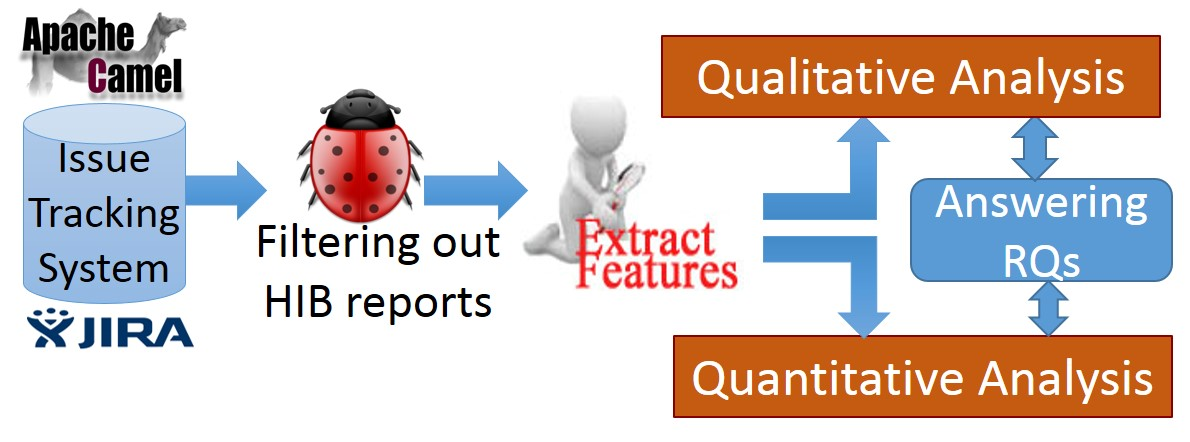
\includegraphics[width=.49\textwidth]{Images/AnalysisP1.jpg}
    \caption{\textsf{Overall HIB reports analysis procedure}}
    \label{fig:AnalP}
  \end{center}
  \end{figure}

\subsubsection{Quantitative Analysis}
In this case study, we also conducted a quantitative analysis to understand whether the request for additional features significantly affects on the bug fixing. In our quantitative analysis, we first divided bug reports into two groups. One group is for additional features request (Res) and another group is for no additional features request (non-Res). Then extract bug report creation date time and bug resolution date time. After that, we calculated bug fixing time for both group. Finally, we applied wilcoxon signed-rank test to know whether the effect of the request for additional features on bug fixing is significant.

 \section{Analysis Result}
This section presents the results for the research question. To get the answers of our research questions first, we carefully examined each reported features in the bug reports. Second, we examined developers and bug reporters each activity to understand the features that developers find useful during bug fixing. Finally, we analyzed the effect of additional request for features on bug fixing.\\

RQ1: What are the features that reporters provide in each type of high-impact bug?\\

The results for the research question 1 are summarized in the figure \ref{fig:RQ1}. 
 \begin{figure*}[t] %[!h] use to make sure position of image like h,t,b=bottom etc.
  \begin{center}
    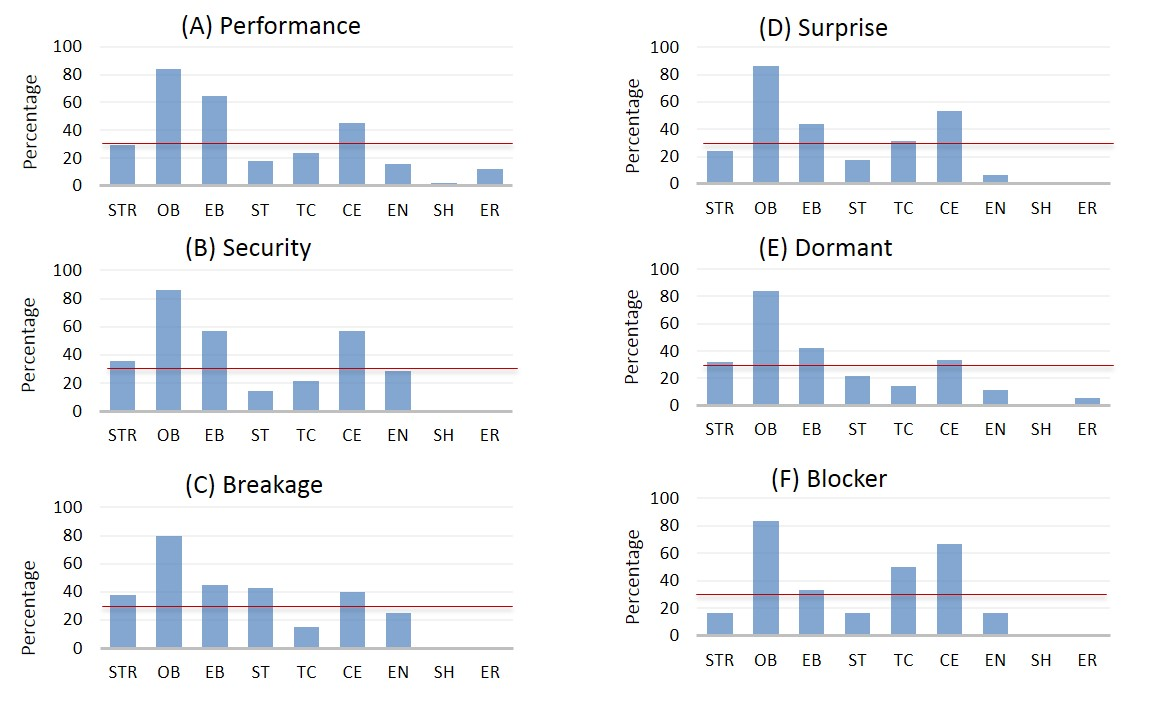
\includegraphics[width=\textwidth , height=13cm]{Images/RQ1_higB3.jpg}
    \caption{\textsf{Observed features in terms of high-impact Bugs}}
     \label{fig:RQ1}
  \end{center}
  \end{figure*}
We see that the average percentages of reported features in Performance, security, Breakage, Surprise, Dormant, and Blocker bug reports are 33\%, 33\%, 32\%, 29\%, 27\%, and 31\% respectively. Whether that is sufficient or not cannot be discussed at this point, since further research on the topic is needed. We also see that the highest percentages of reported features is Observe Behavior among all type of high-impact bugs and Screenshot and Error Report are provided in a very few percentages bug reports. We can see that reporters provided Expected Behavior comparatively in higher percentages in Performance and Security bug reports than others. Other features vary among different types of high-impact bugs.Therefore, at this stage, it is not clear which features have a comparatively higher impact on fixing high-impact bugs than others have. This has lead to the examination of developers and reporters activities during bug fixing for the RQ2  \\

RQ2: Which features did developers request the most during bug fixing in each type of high-impact bugs?\\

To answer this question, we examined each activity and conversation between developers and reporters during bug fixing. We are summarized the analyzed result in the table \ref{table:addrfec}. We found that developers request for additional features on average for 20\% bug reports. Among the 20\% bug reports, in case of Performance bug, 54\% request for Test Cases, 23\% request for Code Example, 15\% request for Steps to Reproduce, and 8\% request for Stack Traces. In our examination, we observed that developers did not make any request to provide additional feature for the blocker bug reports. It does not mean developers do not make additional request for the blocker bug reports. Actually, our analyzed dataset contains a small number of blocker bug reports. We need to analyzed more blocker bug reports to get the actual picture. However, this result can be a good source to understand the useful features that play an important role to fix the high-impact bugs because developers request only for those features that are really helpful for them to localizing and fixing the bugs correctly.

\begin{table}[t]
\caption{Additionally requested features during bug fixing in the high-impact bug reports}
\label{table:addrfec}
\begin{center}
\begin{adjustbox}{width=.49\textwidth}
\begin{tabular}{|c|c|c|c|c|c|c|}
\hline
\multirow{2}{*}{Features} & \multicolumn{6}{ |c| } {High-impact bugs}  \\
\cline{2-7}
 & Performance & Security & Breakage & Surprise & Dormant & Blocker \\
\hline
STR & 15\% & 50\% &9\% & 14\%  & 0\% & 0\%\\
\hline
OB & 0\% & 0\% &0\% & 0\%  & 0\% & 0\%\\
\hline
EB & 0\% & 0\% &0\% & 0\%  & 0\% & 0\%\\
\hline
ST & 8\% & 0\% &0\% & 14\%  & 13\% & 0\%\\
\hline
TC & 54\% & 0\% &55\% & 52\%  & 50\% & 0\%\\
\hline
CE & 23\% & 50\% &27\% & 19\%  & 38\% & 0\%\\
\hline
EN & 0\% & 0\% &0\% & 0\%  & 0\% & 0\%\\
\hline
SH &  0\% & 0\% &0\% & 0\%  & 0\% & 0\%\\
\hline
ER &  0\% & 0\% &0\% & 0\%  & 0\% & 0\%\\
\hline
\end{tabular}
\end{adjustbox}
\end{center}
\end{table}

RQ3: What are the effects of the request for additional features on bug fixing time in high-impact bugs? 
 
To answer this question, we first divided bug reports into two groups. One group is for additional features request (Res) and another group is for no additional features request (No-Res). Then,  we extracted the bug report creation date time and the bug resolution date time. After that, we calculated bug fixing time for both groups. The figure \ref{fig:RQ2_IARvsnonR} shows the distribution of bug fixing time among additional features request and no-request groups. 

 \begin{figure}[t] %[!h] use to make sure position of image like h,t,b=bottom etc.
  \begin{center}
    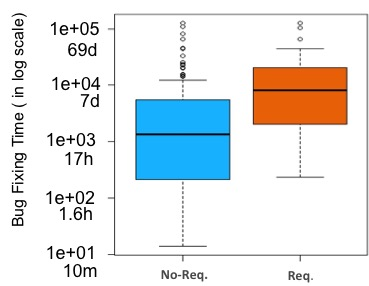
\includegraphics[width=.49\textwidth]{Images/BugFixingTime.jpg}
    \caption{\textsf{Distribution of bug fixing time between additional features request and no-request groups}}
    \label{fig:RQ2_IARvsnonR}
  \end{center}
  \end{figure}

We observed that the median bug fixing time of additional features requested group is comparatively higher than the no-request. Therefore, we conducted a Wilcoxon signed-rank test, to know whether the effect for the request of additional features on bug fixing time is significant. In the test, our null hypothesis $H_0$ and alternative hypothesis Ha are as follows:

$H_0$: There is no statistical difference in bug fixing time between the additional features request and no-request groups.

Ha :The bug fixing time of the additional feature request group is statistically higher than the no-requested group.

The null hypothesis $H_0$ can be rejected and the alternative hypothesis Ha will be accepted when p-value of the statistical test is below the standard significant value, i.e.,  < 0.05. In this study, the Wilcoxon signed-rank test, a non-parametric statistical hypothesis test, was used. This test was selected because the distribution of bug fixing time does not follow a normal distribution. As an outcome of the significant test, we got p-values is 0.000063. It indicates that the request for additional features significantly affects on bug resolution. 
\section{Discussion}
This section discusses some of our major findings from our case study.
 
In our first analysis (RQ1), we find out the frequently reported features across all types of high-impact bugs. We did not consider the features that provided by reporters after initial submission. We have analyzed fixed bug reports in this case study. So, we may consider the most frequently reported features are more useful to fix high-impact bugs than others are. However, at this stage, it is not clear whether they are really useful or not. This has lead to doing the second analysis.\\

In our second analysis (RQ2), we carefully examined developers and reporters each activity during bug fixing. Usually, developers request only for those features during bug fixing that are really helpful. Sometimes, they can not work without them. In this point of view, we can consider that additionally requested features are more useful to developers and have a higher impact on bug fixing. We found that developers made additional request for Test Cases, Code Examples, Steps to Reproduce, and Stack Traces are higher than others. Therefore, we can consider these four are key features for fixing high-impact bugs.\\

In our third analysis (RQ3), we tried to understand whether the request for additional features significantly affects on bug fixing time. Our significant test results suggest that the request for additional features significantly affects on bug fixing time. We tried to find out the reasons by analyzing each additionally requested features, requested time, and response time. We found that developers start working to fix the bug and find missing features that are essential to fix. Then, developers  make the request for additional features to reporters and pause the bug fixing activities until the response of reporters. In many cases, reporters take a long time to response the request. This is the reason to affect the request for additional features significantly on bug fixing. Our case study findings will help to reduce the additional request during bug fixing. Findings from the case study will also help to develop automatic tools. If the reporters do not provide key features in the bug report then the tool may generate an automatic suggestion report to notify what additional features should be included in the bug reports. It also helps to write standard guideline on how to fill-up high-impact bug report so that reporters can submit more accurate bug reports in the bug tracking system (BTS). 

 \section{Threats to Validity}
 For our case study we identified the following threats to validity.

 We examined high-impact bug reports of Apache Camel Project from Jira in our case study. There are some other bug tracking systems (BTS) such as Bugzilla. Every BTS follows their own convention and style to create and store bug reports. So, our finds may vary for the projects of others BTS.

We conducted a case study on high-impact bug reports and normal bug reports of MSR 2015 data showcase paper dataset. The data set contains limited number of high-impact bug reports. So, our result may not be fully representative of their perspective.
 
We have analyzed high-impact bug reports as well as other bug reports of open source projects. Sometimes, proprietary software differ from open source project. In this regard, our findings from this case study might not be applicable to the proprietary projects. We need to analyze OSS projects as well as corporate projects to verify the generality of our findings.
\section{Related Work}
Although we did not find any studies that directly research the topic of key features that play important role to fix high-impact bugs, we did find several studies that are related to our works.
Bettenburg et al.~\cite{Bettenburg:2008} surveyed among 156 experience developers and reporters of Apache, Eclipse and Mozilla to examine what features developers expect to see in the bug reports when fixing bugs. Based on the feedback of developers, they revealed the top 10 most important features that developers find useful during bug fixing. However, they did not investigate actual bug reports to find the usefulness of features. In our empirical case study, we used their survey result to understand how often reporters provide the 10 most important features in the bug reports and to how developers find them useful to fix the bugs. 
	
Steven Davies et al.~\cite{Davies:2014} conducted a case study on four open-source projects (Eclipse, Firefox, Apache HTTP, and Facebook API) to understand what information reporters provide in bug reports. They found that bug reports are neither complete nor accurate, and often do not provide all the information that developers find useful when fixing bugs. Furthermore, they also found that 12 percent of the total information are provided after initial submission of the bug reports. As a result, developers spend their valuable time to collect require information. However, in our case study, we especially focus on high-impact bug reports to reveal the features that developers find most useful during fixing by analysis reported features in the bug reports and conversation between developers and reporters during bug fixing. We also conducted a quantitative analysis to reveal how the request for additional features affects on bug fixing. 

Shahed Zaman et al.~\cite{Zaman:2011} conducted a case study on Firefox project and studied how performance differ from security bugs in a software project. Authors found that security bugs are fixed and triaged much faster, but are reopened and tossed more frequently. Authors considered bug resolution time, triaging time, no. of reopen bug, developers experiences, no. of files changes etc. to make comparison between performance and security bugs. However, our concern about how to file a high-impact bug reports more accurately. 

Several studies used bug reports to automatically assign developers
to bug reports~\cite{Anvik:2006}, assign locations to bug reports~\cite{Canfora:2006}, and predict effort for bug reports~\cite{Weiss:2007}. All these approaches should benefit
by our case study because, the performance of their model affect on the quality of the bug report.

\section{Conclusion \& Future Work}
In this research, we conducted a case study on high-impact bug reports of Apache Camel project to mine insightful information by analyzing reporters and developers activities. We manually analyzed each high-impact bug reports and extract reported features. Then, we examined developers and reporters each activity during bug fixing. From our investigation, it is clear that in many cases, bug reports are not complete or accurate, and often do not provide
features that developers would wish to find, or could use to fix bugs. We found that around 20\% high-impact bug reports collect require features by making the additional request that causes significantly delay on bug fixing. We also found that developers make the additional request for Test Cases, Code Examples, Steps to Reproduce, and Stack Traces comparatively higher that others. Our case study findings suggest that reporters should submit high-impact bug reports more accurately in order to promote the bug-fixing process. Our findings will be helpful to develop automatic tools recommending the bug reporters about the additional features that should be included in the high-impact bug reports. It will also help to formulate guidelines for reporters how to fill up bug report form more accurately. In future, we will conduct a more comprehensive qualitative and quantitative study on different dimensional projects to generalize our case study findings. We also have a plan to work on proposing a novel approach to extract features automatically from the bug report using natural language techniques.


% conference papers do not normally have an appendix


% use section* for acknowledgment
\section*{Acknowledgment}
The authors would like to thank...
\bibliographystyle{IEEEtran}  
\bibliography{SanerEra}  

% that's all folks
\end{document}


